\documentclass{beamer}
%\usepackage{split}

\usepackage{amsmath}
\usepackage{amsfonts}
\usepackage{braket}
\usepackage{subcaption}
\usepackage{tikz}
\usepackage{xcolor}
\usepackage{svg}
\usetikzlibrary{positioning,shapes,arrows.meta}
%\usetikzlibrary{positioning,fit,backgrounds}
\usepackage{quantikz}
\usepackage[linesnumbered]{algorithm2e}
\usepackage{hyperref}
%\usepackage{hyperref,xcolor}
%\usepackage[ocgcolorlinks]{ocgx2}
\usepackage{cleveref}
\usepackage[backend=biber,style=alphabetic,sorting=ynt]{biblatex}
\addbibresource{./sample.bib}


\input{newcommands}


\newcommand*{\QACze}{ \mathbf{QAC}_{0} }
\newcommand*{\QNCzef}{ \mathbf{QNC}_{0,f} }
\newcommand*{\QNCze}{ \mathbf{QNC}_{0} }
\newcommand*{\QNCon}{ \mathbf{QNC}_{1} }
\newcommand*{\NCon}{ \mathbf{NC}_{1} }
\newcommand*{\noiseQNCon}{ noisy-$\QNCon$ }
\newcommand*{\QNC}{ \mathbf{QNC} }
\newcommand*{\QNCG}{ \mathbf{QNC_G} }
\newcommand*{\NC}{\mathbf{NC}}
\newcommand*{\QNCiG}{\mathbf{QNC_{G,i}}}





\usetikzlibrary{patterns, shapes.arrows}
\usepackage{tkz-graph}
\usetikzlibrary{decorations.pathmorphing}
\usepackage{tkz-berge}

\usetikzlibrary{intersections}

\usepackage{cancel}
\begin{document} 

\newcommand*{\Tr}{\textbf{Tr }}


\begin{frame}
  \title{Bounded Communication Fault Tolerance}
    \author{David Ponarovsky}
    \date{\today}
    \titlepage
\end{frame}


\begin{frame}

\frametitle{Introduction}
\begin{block}{Today:}
\begin{itemize}
  \item Bounded Communication Fault Tolerance
    \begin{enumerate}
      \item Walktrough the math 
      \item Alternative definition to Expander decomposition 
      \item $(d,k)$ - Toric 
    \end{enumerate}
  \item New experimental results.  
  \item Answering the code teleportation.  
\end{itemize}
\end{block}
\end{frame}

% ------------------------------------------------ $ 
\begin{frame}
  \frametitle{Bounded Communication Fault Tolerance} 

  \begin{block}{Setting}
    We allow a non-nosy, strong as we wish, classical computation aside. Yet we would like to limit the communication to a constant number of bits per logical qubit, in each round.
\end{block}

\begin{block}{Justification}
  \begin{enumerate}
    \item<+-> If we don't have a constant overhead in depth, in that model, $\Rightarrow$ we also don't have it in the standard model. 
    \item<+-> In that model, gate teleportation for a constant dimension code is easy. Namely, for the Topological codes the task is reduced to finding a decoding with a constant-size hint.  
  \end{enumerate}
\end{block}

\end{frame}


\begin{frame}
  \frametitle{ Max Color } 

\begin{figure}[h]
  \begin{center}
  \tikz{ 
    \node  (A) at (1,0) { Given - $\rho$ };
    \node  (B) at (5,0) { Decoding };
    \node  (C) at (9,0) { $p$-depololraized };
    \draw[->] (A) to (B); 
    \draw[->] (B) to (C); 

    \node  (E) at (1,-1) { $E_{1}$ };
    \node  (D) at (5,-1) { $E_{2}$ };
    \node  (F) at (9,-1) { $E_{3}$ };

    \draw[->] (A) to (E); 
    \draw[->] (B) to (D); 
    \draw[->] (C) to (F); 
  }
\end{center}
\caption{Illustration of the cycle.}
\end{figure}

\end{frame}


\begin{frame}
  \begin{figure}[h]
    \begin{subfigure}[h]{0.4\textwidth}

    \label{alg:three}
    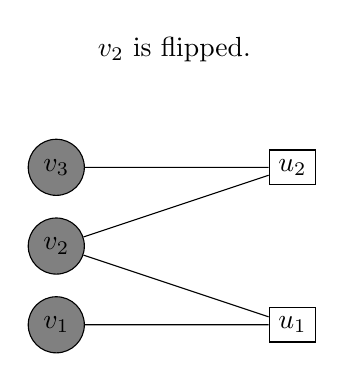
\begin{tikzpicture}%[scale=2.5]
      \draw node at (1.5,4.5) {$v_{2}$ is flipped.};

      \draw node (v0) at (3,1) [draw,shape=rectangle]{$u_1$};
\draw node(v6) at (3,3) [draw,shape=rectangle]{$u_2$};
\draw node foreach \x in {1,3} (v\x) at (0,\x) [draw,shape=circle, fill=gray]{$v_\x$};
\draw node (v2) at (0,2) [draw,shape=circle, fill=gray]{$v_2$};
\draw (v0) -- (v1)
  (v0) -- (v2)
  (v6) -- (v2)
  (v6) -- (v3);
\end{tikzpicture}
    \end{subfigure}
    \begin{subfigure}[h]{0.1\textwidth}
      \
    \end{subfigure}
    \begin{subfigure}[h]{0.45\textwidth} 

    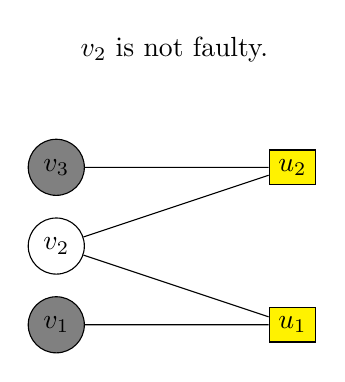
\begin{tikzpicture}%[scale=2.5]
      \draw node at (1.5,4.5) { $v_{2}$ is not faulty.};
      \draw node (v0) at (3,1) [draw,shape=rectangle, fill=yellow]{$u_1$};
      \draw node(v6) at (3,3) [draw,shape=rectangle, fill=yellow]{$u_2$};
\draw node foreach \x in {1,3} (v\x) at (0,\x) [draw,shape=circle, fill=gray]{$v_\x$};

\draw node (v2) at (0,2) [draw,shape=circle]{$v_2$};
\draw (v0) -- (v1)
  (v0) -- (v2)
  (v6) -- (v2)
  (v6) -- (v3);
\end{tikzpicture}
    \label{fig:location}
    \end{subfigure} 
  \end{figure}


  If the majority of bits in the local view of $v_{2}$ are flipped, then after decoding, $v_{2}$ will be also (remain) flipped.

\end{frame}


\begin{frame}
  \frametitle{Strategy}
Suppose we have the following Lemma: 
\begin{block}{Nice To Have Lemma.} There is a function $f : [2^{n}] \rightarrow \mathbb{R}$, such that for any (encoded) $\rho$ which is subjected to $q$-local stochastic noise and a subset of qubits $S$ we have:  
    \begin{enumerate}
      \item With high probability ($1 - e^{-\sqrt{n}}$), after the decoding stage, the probability that the error is (partly) supported on $S$ is bounded by $C \cdot q^{f(|S|)}$
      \item $f(|S|) \ge \alpha|S|$ for some $\alpha > 0$. 
    \end{enumerate}
  \end{block}
\end{frame}

\begin{frame}
  \frametitle{Strategy}
  The Nice-To-Have-Lemma implies that after decoding $+$ absorbing $p$-depolarized noise, we have with high probability:  
  \begin{align*}
    \prb{S} &  \le \sum_{S^{\prime} \subset S }{C\cdot q^{f(S^{\prime}) }p^{|S /S^{\prime}|}  } \le C \cdot \left( q^{\alpha} + p \right)^{|S|} \le C \cdot q^{|S|}
  \end{align*}
\end{frame}

\begin{frame}
  \frametitle{Strategy}
  %\begin{block}{Demonstration on the classical case.}
  Consider the classical expander code, defined via bipartite expander graph. The Tanner graph consists two subsets of checks $C_{+}$ and $C_{-}$, such that checks in each subset don't share bits. Each of the bits is connected to one check in $C_{-}$ and one check in $C_{+}$.


  Then 

    $(\gamma,\varepsilon)$- expander Tanner graph. Namely, each subset on left at size at most $\gamma n$ sees $(1-2\varepsilon)\Delta$ uniq checks (checks that connected by single edge to the subset).
   % \end{block}

  \begin{align*}
    \prb{S} &  \le \sum_{S^{\prime} \subset S }{C\cdot q^{f(S^{\prime}) }p^{|S /S^{\prime}|}  } \le C \cdot \left( q^{\alpha} + p \right)^{|S|} \le C \cdot q^{|S|}
  \end{align*}
\end{frame}
\begin{frame}
  \frametitle{SWIFT}

  \begin{block}{What did we learn?}
\begin{enumerate}
  \item Storing time is, likily, not $\Theta(e^{n})$, might be $\Theta(L^{\alpha})$ for $\alpha \in (0,1)$.   
  \item $ \Rightarrow $  Implies that the structure of the theorem/key-lemma is different than the known refrigerators.  
\end{enumerate}
  \end{block}
\end{frame}

\begin{frame}
  \frametitle{Future}
 \begin{block}{So What's Next?}
   \begin{enumerate}
     \item<+-> Moving forward with the experimental work? 
       \begin{itemize}
         \item More experiments, higher statistical standards?
         \item Accelerate the decoder? Shifting to \textit{c/c++}? Parallelize it with GPUs? Do we have budget? 
         %\item Publishing 'A Tale of Five Decoders'?
       \end{itemize}
     \item<+-> Dividing to colors - Expander Decomposition? What do we know about the expander decomposition of the periodic grid? 
     \item<+-> How to use the fact our code is a quotient code? 
   \end{enumerate}
 \end{block}
\end{frame}


\end{document}
